\documentclass[a4paper,11pt]{article}
\usepackage[utf8]{inputenc}
\usepackage[T1]{fontenc}
\usepackage{helvet}
\renewcommand{\familydefault}{\sfdefault}

\usepackage{titlesec}
\titlespacing*{\section}{0pt}{*1.5}{*1.5} % Abstand vor und nach \section anpassen
\titlespacing*{\subsection}{0pt}{*1.5}{*1.5}
\usepackage{geometry}
\usepackage{fancyhdr}
\usepackage{setspace}
\usepackage{lipsum} % Zum Einfügen von Beispieltext
\usepackage{hyperref}
\usepackage{chngcntr}
\counterwithout{footnote}{section}
\counterwithout{figure}{section}
    \counterwithout{table}{section}
% Seitenränder
\geometry{a4paper, left=2cm, right=2cm, top=2cm, bottom=2cm}

% Überschriftenformatierung
\titleformat{\section}
  {\normalfont\fontsize{12}{15}\bfseries}{\thesection}{1em}{}

% Zeilenabstand
\onehalfspacing

% Blocksatz und Silbentrennung
\usepackage[ngerman]{babel}
\usepackage{hyphenat}
\hyphenation{Sil-ben-tren-nung}

\usepackage{caption}
\captionsetup[figure]{name=Abb., labelsep=space}

% Fußnotenformatierung
\renewcommand{\footnotesize}{\fontsize{10}{12}\selectfont}
\usepackage{ragged2e}
\justifying

% Seitenzahlen
\pagestyle{fancy}
\fancyhf{}
\fancyfoot[C]{\thepage}
\renewcommand{\headrulewidth}{0pt} % Remove the header line

% Römische Seitenzahlen für vordere Seiten
\pagenumbering{Roman}

% Abstand nach Absätzen
\usepackage{parskip}
\setlength{\parskip}{6pt}

% get custom bibliography style working without prepending [brackets]
%\usepackage{natbib}
%\setcitestyle{aysep={}} % remove comma as delimiter  
\usepackage[utf8]{inputenc} %UTF-8 to encode many characters => for many characters, you can just input the character and avoid a macro
\usepackage{csquotes} % Recommended when using biblatex with babel/polyglossia
\usepackage[style=apa, backend=biber]{biblatex}
\DeclareLanguageMapping{ngerman}{ngerman-apa} % falls du babel ngerman nutzt
\addbibresource{biblio.bib}

\AtBeginBibliography{%
  % Oxford comma aus (bei 3+ Autoren)
  \renewcommand*{\finalandcomma}{}%
  % Kein Komma vor "&" in der Literaturliste
  \DeclareDelimFormat{finalnamedelim}{\addspace\&\space}%
}

\usepackage{float}
\usepackage{graphicx}
\usepackage{placeins}

\usepackage{pgfplots}
\pgfplotsset{compat=1.18}
\usepackage{pgfplotstable}

\usepackage[withpage]{acronym}

\usepackage{tikz}
\usetikzlibrary{shapes.geometric, arrows}
\tikzstyle{startstop} = [rectangle, rounded corners, minimum width=3cm, minimum height=1cm,text centered, draw=black, fill=white!30]
\tikzstyle{process} = [rectangle, minimum width=3.5cm, minimum height=1cm, text centered, draw=black, fill=white!10]
\tikzstyle{arrow} = [thick,->,>=stealth]


\begin{document}

% Ab hier römische Seitenzahlen
\setcounter{page}{1}
\pagestyle{fancy}

% Arabische Seitenzahlen für den Textteil
\pagenumbering{arabic}

\section{Konzeptionsphase}

\textbf{Ziel der Arbeit} ist die Konzeption und Umsetzung einer Cloud-Architektur für eine einfache Unternehmenswebsite.
Die Anwendung muss hochverfügbar betrieben werden, weltweit mit geringer Latenz erreichbar sein und ein Backend automatisch,
anhand von Zugriffszahlen, skalieren können. Für den Zweck dieses Projekts wird eine einfache .html als Webseite dienen.  

\textbf{Ausgangsidee und Tragfähigkeit.} Der zentrale Gedanke ist, die Website in einem Container bereitzustellen.
Ein Edge-Dienst soll sich dann um die Verteilung des Traffics kümmern.
Für die Wahl von Azure spricht, dass keine Kreditkarte zwingend erforderlich ist und sich moderne, managed Dienste für globales Routing und autoskalierendes Hosting kombinieren lassen.
Gegen die Idee könnte sprechen, dass Containerbetrieb für eine rein statische Seite technisch anspruchsvoller als nötig ist.
Dennoch ist dieser Ansatz tragfähig, da er als Lernziel dient und später ein echtes Backend ohne grundlegende Plattformänderung ergänzt werden kann.

\textbf{Konzept und Architektur.} Die Zielarchitektur besteht aus fünf Kernbausteinen:
\begin{itemize}
    \item \textbf{GitHub} als Quellcodeverwaltung
    \item \textbf{GitHub Actions} als CI/CD-Pipelineeee
    \item \textbf{Azure Container Registry (ACR)} als Container-Image-Registry
    \item \textbf{Azure Container Apps (ACA)} in zwei Regionen als Hosting-Layer mit automatischer Skalierung
    \item \textbf{Azure Front Door} als globaler Entry-Point, der Anfragen weltweit entgegennimmt und zur nächstgelegenen Region routet
\end{itemize}
Damit wird globale Performance erreicht und gleichzeitig die Hochverfügbarkeit durch Multi-Region-Betrieb erhöht.
Die Skalierung erfolgt in ACA über konfigurierbare Minimum-/Maximum-Replikas und HTTP-basierte Skalierungsregeln.
Bei Lastspitzen werden automatisch zusätzliche Containerinstanzen gestartet, bei geringer Last wieder reduziert.
Das beiliegende Architekturdiagramm visualisiert diese Komponenten und deren Interaktion.

\textbf{Ablauf.} 
Der Ablauf in der Pipeline ist wie folgt: Bei einem Push auf den \texttt{main}-Branch baut GitHub Actions ein Docker-Image aus der HTML-Datei,
pusht dieses in die ACR und führt \texttt{terraform apply} aus, um (a) ACR, (b)
Container Apps in zwei Regionen und (c) Azure Front Door inklusive Routing zu erstellen oder zu aktualisieren.
Die Website ist anschließend über die Front-Door-URL erreichbar, wobei Front Door die Anfragen global verteilt und ACA die Containerzahl
automatisch anpasst.

\textbf{Methodik/Tooling und Begründung.} Terraform wird gewählt, weil es Cloud-Ressourcen deklarativ beschreibt, Änderungen nachvollziehbar
macht und die Reproduzierbarkeit der Architektur sicherstellt. GitHub Actions ergänzt dies als automatisierter Delivery-Prozess,
der Quellcodeänderungen ohne manuelle Zwischenschritte in ein deploybares Artefakt (Container-Image) und eine konsistente Infrastruktur überführt.
Insgesamt erfüllt das Konzept die geforderten Eigenschaften (Hochverfügbarkeit, globale Performance, Autoscaling) und ist gleichzeitig so
ausgerichtet, dass ein späteres Backend als zusätzliche Container App mit Front-Door-Routing integriert werden kann.

\begin{figure}[h]
\centering
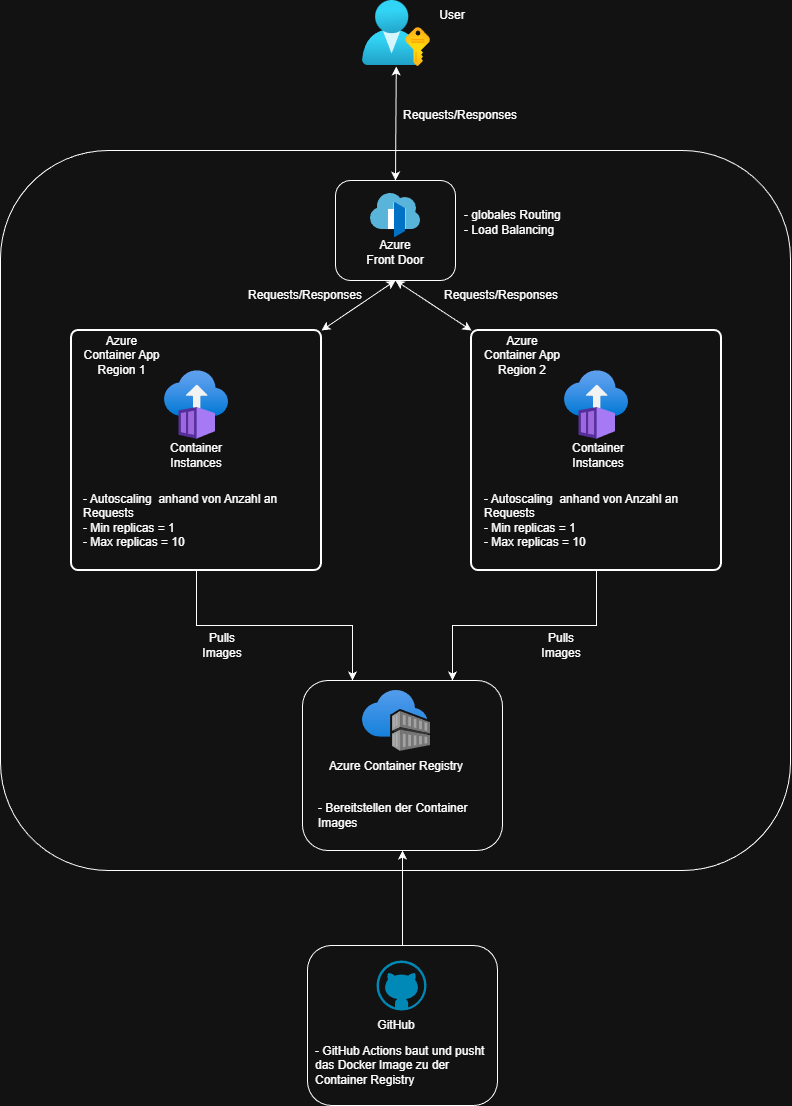
\includegraphics[width=1\textwidth]{pics/CloudArchitecture.png}
\end{figure}

\end{document}